
\section{Concepción}

El objetivo de este documento es recoger todos los aspectos relacionados
con la concepción del proyecto 
\emph{SWAML, publicación de listas de correo en web semántica}, realizando
para ellos una captación de requisitos para su posterior análisis.

\subsubsection{Documentos recogidos}

\begin{itemize}
 \item Visión
 \item Especificación de requisitos
 \item Especificación de casos de uso
 \item Especificaciones secundarias
 \item Plan del proyecto
\end{itemize}


\subsection{Visión}

Como ya se comentó en los objetivos recogidos en el capítulo destinado a
la memoria del proyecto, se tiene como objetivo principal la publicación 
de los archivos antigüos de listas de correo en un formato rico 
semánticamente.

De esta manera esta inmensa base de conocimiento podrá ser procesada a 
posteriori por aplicaciones ya existente o nuevas aplicaciones que 
\emph{exploten} dicho entiquecimiento semántico. Esta ya es un área de 
actuación sólo contemplada parcialmente en el proyecto.

\subsubsection{Situación actual}

Dado que que no existe en la actualidad ninguna solución software que
resuelva el problema, la herramienta cubriría una serie de necesidades
aún sin explotar, que seguramente abran un nuevo camino a nuevos 
desarrollos en este campo.

\subsubsection{Descripción del problema}

Se pretende solucionar un problema principalmente:

\begin{itemize}
  \item \textbf{El problema de} exportar semánticamente los archivos 
	de una lista de correo.
  \item \textbf{Afecta a} los usuarios que habitualmente utilizan los 
	archivos de estas listas de correo como completa fuente de 
	información.
  \item \textbf{Lo que implica} es obtener de mbox todos los mensajes 
	y sus relaciones, para poder publicarlas sin apenas pérdida de
	información.
  \item \textbf{Una solución adecuada haría que} fueran muchos más
	explotables estos datos, permitiendo por ejemplo busquedas
	mucho más completas y fiables.
\end{itemize}

\subsubsection{Descripción de los usuarios}

El software tendrá dos tipos de usarios muy claramente identificados:

\begin{enumerate}
  \item \textbf{Usuario administrador:} será la persona encargada de
	instalar el software y parametrizarlo para que realice su
	función según sus necesidades particulares. Evidentemente debe
	ser un usuario avanzado con conocimientos básicos de administración
	de sistemas.
  \item \textbf{Usuarios convencionales:} los usuarios que \emph{consuman},
	bien con alguna aplicación genérica u otroa cualquiera hecha a medida,
	el conocimiento generado para cubrir una necesidad concreta. No
	tendrían, en principio, que necesitar tener ningún conocmiento 
	sobre la materia, ni siquiera fuertes conocmientos informáticos.
\end{enumerate}

\subsubsection{Resumen de capacidades}

A continuación se identifican las capacidades del producto en términos de 
beneficios para el usuario y la caracteristica que lo proporciona:

\begin{itemize}
  \item \textbf{Recomponer la lista de correo:} se podrá recomponer, filtrando 
	previamente por múltiples parámetros como fecha o tema, los hilos de una 
	lista de correo sin necesidar de estar suscrito a ella
  \item \textbf{Obtener más información de los suscriptores:} apoyandose por 
	ejemplo en FOAF, se podrán conocer muchos detalles de los suscriptores 
	que la lista de correo no contiene en su formato original.
  \item \textbf{Mejora de la accesibilidad:} intrinsicamente al describir muy 
	ricamente el contenido, le será muy fácil interpretar correctamente 
	la información a los agente de usuario para personas que sufren algún 
	tipo de discapacidad.
\end{itemize}

\subsubsection{Calidad exigida al producto}

Se definen unos rangos de calidad respecto a eficiencia, robustez, 
tolerancia a fallos, facilidad de manejo y características similares 
del sistema software a desarrollar.

\begin{itemize}
  \item \textbf{Disponibilidad:} el software generará una base del 
	conocimiento que debe estar accesible de forma continua.
  \item \textbf{Escalibilidad:} la arquitectura general del sistema 
	será lo suficientemente flexible para soportar un amplio
	rango en los datos que pueda manejar, siendo extremadamente
	recomendable contemplar optimizaciones de generación de los 
	datos de forma incremental.
  \item \textbf{Mantenimiento:} evidentemente tanto la solución software 
	como en los datos generados se ha de tener muy en cuenta su
	mantenibilidad.
\end{itemize}







\subsection{Especificación de requisitos}

Debido a la naturaleza del problema a resolver la \textbf{introspección}
ha sido la técnica usada para realizar la captura de requisitos software.

Esta técnica recomienda que sea el propio ingeniero de requisitos quien 
se ponga en el lugar del cliente y trate de imaginar como desearía él el 
sistema. Y en base a estas suposiciones comenzar a recomendar al cliente 
sobre la funcionalidad que debería presentar el sistema. El problema radica 
en  que un ingeniero no es un tipo normal de cliente, posee un conocimiento 
técnico mas elevado por lo que se podrían recomendar cosas que el cliente 
no necesite.

Pero además circunstancialmente también se hizo uso de la técnica conocida
como las \textbf{entrevistas}, principalmente discusiones. Como adaptación
a las circunstancias concretas fueron ambos co-directores del proyecto 
quienes ejercieron la función del cliente.

\subsubsection{Datos de entrada}

La fuente de información será una lista de correo en formato mbox 
(RFC4155\cite{Hall2005}), un formato estandarizado que utilizan la 
mayoría de los sistemas de gestión de listas de correo, entre otros:

\begin{itemize}
 \item Mailman\footnote{\url{http://www.gnu.org/software/mailman/}}
 \item Majordomo\footnote{\url{http://www.greatcircle.com/majordomo/}}
 \item LISTSERV
 \item Listproc
 \item SmartList
\end{itemize}

El formato mbox no es más que un fichero de texto plano en el que se van
almacenando consecutivamente los correos que van llegando a la lista. Se 
almacenan tal cual son enviados a la lista, con su cabeceras originales 
completas y en la codificación del cliente de correo del usuario.

Por tanto es fácil adivinar dos problemas evidentes de este formato:

\begin{itemize}

  \item \textbf{Identificadores:} cada correo dispone de un identificador 
	(cabecera \texttt{Message-Id}), pero este identificador nadie 
	asegura que sea único.

	Cuando alguien responde un determinado mensaje, el cliente de correo 
	colocará en la respuesta una cabecera (\texttt{In-Reply-To}) con este 
	\texttt{ID} para referirse explícitamente al mensaje que se está 
	respondiendo.

	Este es el mecanismo especificado en el RFC2822\cite{Resnick2001} para 
	la gestión de hilos de conversación por medio de correo electrónico. 
	Y el mecanismo que es utilizado para representar los hilos de 
	conversaciones en forma de árbol, tanto en clientes de correo (Evolution, 
	Thunderbird, Outlook, etc) como en alguno de los sistemas convencionales 
	de publicación de listas de correo nombrados anteriormente.

	Dicho identificador tiene una forma similar a 
	\texttt{<3C94C55A3B6A@smtp.isp.com>}.

	Pero ese ID no es único, sino que es asignado por el propio servidor
	SMTP\footnote{\url{http://es.wikipedia.org/wiki/SMTP}} (Simple Mail 
	Transfer Protocol) del usuario de forma arbitraria a la hora de enviar 
	el correo. Por tanto no debería poder usarse, al menos garantizando un 
	rigurosidad extrema a la hora de identificar cada uno de los mensajes 
	y sus respuestas.

	Podrían usarse algoritmos heurísticos más sofisticados con el asunto del 
	mensaje, aunque tampoco nos garantizarían una fiabilidad absoluta al 
	poder cambiarse el asunto en cualquier mensaje del hilo.

	Pero si existe una aproximación al problema que consigue una efectividad 
	bastante alta según se ha podido comprobar. Consiste en asumir que cuando 
	hay una respuesta a un mensaje, existe una alta probabilidad que se esté 
	respondiendo a último de los mensajes enviados con ID repetido. Empíricamente 
	se ha demostrado que este probabilidad supera el 95\%.

  \item \textbf{Codificación:} un viejo problema de la informática a la hora de 
	interactuar entre varios sistemas. Actualmente dos codificaciones, ISO 
	y Unicode, son las más utilizadas y extendidas.

	El problema radica en la heterogeneidad de codificaciones que utilicen 
	los usuarios. Los sistema de listas de correo no suelen atender a la 
	codificación de los correos que reciben, y los \emph{vuelcan} todos al 
	mbox codificado en la codificación que use el sistema servidor. Ello 
	provoca en muchos casos una corrupción de algunas cadenas, siendo 
	tremendamente difícil recomponerlas de nuevo a la hora de procesarlas.

\end{itemize}

\subsubsection{Datos de salida}

Como el fin principal del proyecto es publicar las listas de correo en un
formato semánticamente rico, es evidente que el formato principal de salida
será \textbf{RDF}.

Pero también se pueden contemplar otros formatos de salida complementarios:

\begin{itemize}
  \item \textbf{(X)HTML}: para su visualización en navegadores convencionales.
	Evidentemente ambos (RDF y HTML) deberán enlazarse mutuamente.
  \item \textbf{KML}: el formato KML 2.0\footnote{\url{http://earth.google.com/kml/kml_intro.html}}
	(Keyhole Markup Language) es una gramática XML para describir determinadas
	características geográficas (puntos, lineas, imágenes, polígonos, etc.)
	que luego pueden ser 
	\emph{explotados}\footnote{\url{http://googlemapsapi.blogspot.com/2006/11/kml-on-google-maps.html}} 
	desde Google Maps\footnote{\url{http://maps.google.es/}} o
	Google Earth\footnote{\url{http://earth.google.com/}}. Por tanto
	puede ser muy interrsante exportar los suscriptores de la lista de
	correo, para así automáticamente poder utilizar esta información
	desde las herramientas que ya existen.
\end{itemize}

\subsubsection{Lenguaje de programación}

El problema planteado requiere de una lenguaje de programación que disponga
de determinadas características:

\begin{itemize}
  \item \textbf{Fácil despliegue:} hay que procurar que SWAML se pueda desplegar 
	en todo tipo de máquinas, sin excesivos requisitos ni hardware ni software.
	Es importante que SWAML pueda ser invocado por los distintos programadores
	de tareas de que disponen los sistemas operativos (cron y similares), pues
	SWAML no será un proceso interactivo sino un proceso por lotes.
  \item \textbf{API para RDF:} que disponga de una madura biblioteca, a poder ser 
	nativa, para manejar RDF (creación de grafos, parseo desde disco/URI, 
	serializado a disco y/o bases de datos, consultas SPARQL, etc).
  \item \textbf{Biblioteca para ficheros mbox}: sería interesante disponer de una 
	biblioteca que abstraiga lo mayor posible al proyecto del manejo de ficheros
	mbox\cite{Hall2005} y mensajes de correo electrónico\cite{Resnick2001}.
\end{itemize}

Por tanto el cumplimiento de estas tres necesidades principales debe ser lo 
primero a valorar entre todos lenguajes de programación candidatos a convertirse 
en el lenguaje utilizado para implementar SWAML. 

Pero también se ha de tener en cuenta otras cualidades más generales al problema,
como por ejemplo:

\begin{itemize}
  \item Aspectos concretos de la OOP (object-oriented programming, programación 
	orientada a objetos) que cubra.
  \item Sencillez de desarrollo y posterior estudio del código.
  \item Portabilidad de la solución generada.
  \item Posibilidad de usarse compiladores/intérpretes libres.
\end{itemize}

Después de revisar los lenguajes disponibles, fueron varios los candidatos para
someterlos a un estudio más profundo:

\paragraph{Java:}Java\footnote{\url{http://java.sun.com/}} es un lenguaje de 
programación, desarrollado por Sun Microsystems, orientado a objetos muy popular 
desde hace varios años. Java no se compila a código nativo, sino que una JVM 
(Java Virtual Machine, máquina virtual de Java) ejecuta el bytecode previamente 
compilado.

En la actualidad se disponen de multitud de implementaciones de la máquina virtual
de Java, desde las propietarias (IBM, HP, etc) hasta las libres (Sun, Harmony, GIJ, 
Kafee, IKVM.NET, etc).

Sobre el problema que nos atañe:

\begin{itemize}
  \item Actualmente las JVM existentes cubren un amplio abanico de arquitecturas y 
	sistemas operativos. Aunque Java esté más pensado para su uso en otro tipo
	de entornos (J2EE por ejemplo), puede invocarse perfectamente en modo en
	linea y resolver problemas de procesamientos por lotes como el que nos
	atañe.
  \item Dispone de forma nativa (desarrollada también en Java) de la biblioteca para
	manejar RDF más madura actualmente: Jena\footnote{\url{http://jena.sourceforge.net/}}.
	El framework Jena incluye paquetes para múltiples propósitos dentro de la web
	semántica: API para RDF y OWL, persistencia, serializado y soporte para consultas
	SPARQL.
  \item Con JavaMail\footnote{\url{http://java.sun.com/products/javamail/}} y
	jmbox\footnote{\url{http://jmbox.dev.java.net/}} se conseguiría un nivel
	de abstracción del problema suficiente para centrarse en el desarrollo
	de las otras capas.
\end{itemize}

En las fechas en que se desarrolló esta especificación de requisitos la máquina virtual
de Java de Sun, la más completa y eficiente actualmente, no era libre. Por tanto en 
aquellas fechas tuvo que ser tomado como un punto negativo, pues complicaría de 
una manera importante un futura distribución de SWAML de manera totalmente libre,
por tener como dependencias paquetes no libres.

Pero la noticia de la liberación de Java por parte de Sun\footnote{\url{http://www.sun.com/2006-1113/feature/story.jsp}} ha obligado a la
revisión de este documento. Si bien las conclusiones de este documento se ven 
desvirtuadas (que Java no fuese libre en esas fechas fue un argumento de peso para
descartarlo como lenguaje), al menos recoger en estas lineas dicha noticia.

\paragraph{Python:}Python\footnote{\url{http://www.python.org/}} es un lenguaje de 
script extremadamente eficiente. Su uso está muy extendido en todos los sistemas 
Unix actuales (GNU/Linux, familia BSD, Solaris, etc), aunque también está disponible\footnote{\url{http://www.python.org/download/}} para la mayoría de sistemas 
operativos actuales (Windows, MacOS y demás).

Se trata de un lenguaje de script mucho más moderno que otros lenguajes hermanos 
tipo bash o perl. Python va más alla, disponiendo en un lenguaje de script 
interpretado y con tipado dinámico de toda la potencia de los lenguajes orientados 
a objetos más modernos.

Respecto a los tres requisitos que nos interesan:

\begin{itemize}
  \item Al tratarse de un lenguaje de script basta disponer de un intérprete 
	instalado en el sistema para poderlo ejecutar. Además esta característica
	simplifica enormemente la forma de invocarlo desde un programador de
	tareas.
  \item Existen varias posibilidades para manejar RDF desde Python. Algunas son
	bibliotecas nativas desarrolladas también en Python, y otras están
	disponibles en forma de bindings a bibliotecas desarrolladas en otro 
	lenguaje.
	De todas las posibilidades\cite{PracticalRDF}, quizás 
	RDFLib\footnote{\url{http://rdflib.net/}} sea la que se encuentra en 
	un estado de desarrollo más avanzado y maduro (persistencia, serialización, 
	consultas SPARQL, etc.).
	Además ofrece la posibilidad de \emph{colocar encima} otras bibliotecas,
	como por ejemplo Sparta\footnote{\url{http://www.mnot.net/sw/sparta/}},
	para utilizar determinados conceptos que no contempla RDFLib.
  \item Python dispone una extensa y completa biblioteca estándar, además de contar
	con multitud de bibliotecas para los más variopintos propósitos. Con módulos 
	como email\footnote{\url{http://docs.python.org/lib/module-email.html}} y
	mailbox\footnote{\url{http://docs.python.org/lib/module-mailbox.html}}, el
	problema de acceso primario a los datos (mailbox unix) que SWAML deberá
	consumir se verá resuelto de manera muy eficiente a un nivel de abstracción
	bastante alto.
\end{itemize}

Además es un lenguaje totalmente libre, desde su especificación hasta varias
de sus implementaciones, incluido el intérprete oficial.

Mailman\footnote{\url{http://www.gnu.org/software/mailman/}}, el sistema de gestión
de listas de correo más popular hoy en día, también está escrito en Python, lo que 
facilitaría en gran medida una posible integración de SWAML en Mailman.


\paragraph{C\#:}C\#\footnote{\url{http://msdn2.microsoft.com/en-us/vcsharp/aa336809.aspx}} 
es un lenguaje de programación desarrollado por Microsoft, y posteriormente estandarizado por el ECMA\footnote{\url{http://www.ecma-international.org/publications/standards/Ecma-334.htm}},
como parte fundamental de su plataforma .NET\footnote{\url{http://www.microsoft.com/net/}}.

\begin{itemize}
  \item Los requerimientos de recursos no parecen que sea la mejor opción para una tarea
	de estas características.
  \item Se dispone de SemWeb\footnote{\url{http://razor.occams.info/code/semweb/}}, una
	biblioteca con un inmaduro soporte para RDF y SPARQL. También están disponibles los 
	bindings a C\# de Redland\footnote{\url{http://librdf.org/docs/csharp.html}}, 
	aunque estos ofrecen un pobre rendimiento.
  \item Por ahora no parece existir ninguna biblioteca que ayude en el parseo de los mailboxes 
	de Unix, aunque no parece complicado su desarrollo dada la cantidad de módulos para 
	manejar formatos de correo de que dispone la plataforma.
\end{itemize}

Dispone además de varias implementaciones libres, como 
Mono\footnote{\url{http://www.mono-project.com/}} o DotGNU\footnote{\url{http://dotgnu.org/}}.
Pero hoy por hoy la implementación más completa es la desarrollada por Microsoft. Usar por 
tanto su framework no sólo complicaría los términos de distribución de SWAML, sino que 
encima coartarían su funcionamiento a las plataformas soportadas actualmente por ese 
framework (únicamente Microsoft Windows).


\paragraph{Perl:}Perl\footnote{\url{http://www.perl.org/}} es un lenguaje de script de 
gran tradición. Soporta paradigmas de programación imperativos (estructurados y orientados 
a objetos) y lógico-funcionales.

\begin{itemize}
  \item Está especialmente extendido en sistemas Unix y, en menor medida, en sistemas
	operativos Windows. Sus requerimientos son realmente bajos y, dada su naturaleza
	de script, está especialmente pensado para invocarse en linea.
  \item Con RDFStore\footnote{\url{http://rdfstore.sourceforge.net/}} se dispone de un 
	API bastante bueno para manejar RDF desde Perl. También existe una
	implementación\footnote{\url{http://www.w3.org/1999/02/26-modules/}} 
	desarrollada por el W3C para manejar RDF desde Perl. Aunque ni es una implementación
	demasiado completa ni es un proyecto mantenido en la actualidad.
  \item En CPAN\footnote{\url{http://www.cpan.org/}} hay disponibles multitud de bibliotecas
	y módulos útiles para hacer desarrollos en Perl. Entre ellas está
	MessageParser\footnote{\url{http://search.cpan.org/~dcoppit/Mail-Mbox-MessageParser-1.4005/lib/Mail/Mbox/MessageParser.pm}},
	que podría ser una perfecta candidata para resolver en Perl este problema.
\end{itemize}

En su contra juega su sintaxis excesivamente críptica, que hacen muy complicada
la lectura y/o reescritura del código.

\paragraph{Ruby:}Ruby\footnote{\url{http://www.ruby-lang.org/}} es un lenguaje de 
programación interpretado orientado a objetos con quince años de historia, que 
recientemente se ha hecho más popular por la aparición del framework web 
Ruby on Rails\footnote{\url{http://www.rubyonrails.org/}}. Con una sintaxis muy
parecida a Perl con detalles de Smalltalk.

\begin{itemize}
  \item Sus dos principales interpretes, Ruby y JRuby, están disponibles para la
	mayoría de plataformas actuales. Sus requerimientos son realmente bajos y
	sus rendimiento notable en las últimas versiones.
  \item RubyRDF\footnote{\url{http://www.w3.org/2001/12/rubyrdf/intro.html}} y 
	Rena\footnote{\url{http://raa.ruby-lang.org/project/rena/}} están aún
	realmente verdes, y los bindings de Redland\footnote{\url{http://librdf.org/docs/ruby.html}} 
	ofrecen un rendimiento bastante pobre.
  \item RubyMail\footnote{\url{http://www.lickey.com/rubymail/}} podría servir,
	aunque parece que la biblioteca se encuentra abandonada en los últimos años. 
	Algo parecido ocurre con mbox\footnote{\url{http://raa.ruby-lang.org/project/mbox/}}.
\end{itemize}

\paragraph{Conclusión:}Una vez estudiadas y evaluadas cuidadosamente todas estas 
alternativas, se llegó a la conclusión de que Python era el lenguaje que mejor se 
adaptaba a los requisitos del proyecto. Tanto por cumplir los tres requisitos 
no funcionales principales buscados, como por ser un lenguaje moderno y flexible 
que permitirá manejar de una forma muy cómoda todos las estructuras de datos que se
necesitarán.

La documentación es variada, desde la propia página Web oficial del 
lenguaje\footnote{\url{http://www.python.org/}} hasta la gran cantidad de libros
que hay disponibles (\emph{Learning Python}\cite{LearningPython},
\emph{Python Essential Reference}\cite{PythonEssential}, 
\emph{Dive into Python}\cite{DivePython} o \emph{Python Pocket Reference}\cite{PythonPocket},
por ejemplo).



\subsection{Especificación de casos de uso}

Este documento contiene la descripción de los casos de uso. El modelo 
de casos de uso es un modelo de las funciones que realiza el sistema y 
su entorno, y sirve de contrato entre el cliente y los desarrolladores. 
Se emplea como entrada para las actividades de análisis, diseño y test.

Este documento contiene además aquellos requisitos que no pueden ser 
obtenidos tan solo con un análisis basado en casos de uso, como los 
requisitos de rendimiento o fiabilidad.

\subsubsection{Actores}

Un actor define un conjunto coherente de roles que los usuarios del 
sistema interpretan cuando interactúan con el mismo. Puede ser un 
individuo o un sistema externo.

Se procederá a enumerar los actores que participan en el sistema, 
así como una breve descripción de cada uno de ellos.

\begin{itemize}
  \item \textbf{Usuario:} Representa a la persona que interacturá con 
	la base del conocimiento generada. No manipulará los datos, 
	sino que los usará para hacer consultas y/o busquedas.
  \item \textbf{Administrador:} Representa al usuario que se encargue 
	de administrar el servicio y la máquina que lo aloje. Su labores 
	principales serán la de programar actualizaciones y verificar 
	que hayan resultado satisfactoriamente.
\end{itemize}

\subsubsection{Límites del sistema}

En la figura siguiente se establecen los límites del sistema, así 
como los principales casos de uso que posteriormente serán refinados 
en siguientes etapas del análisis.

\begin{figure}[ht]
 	\centering
	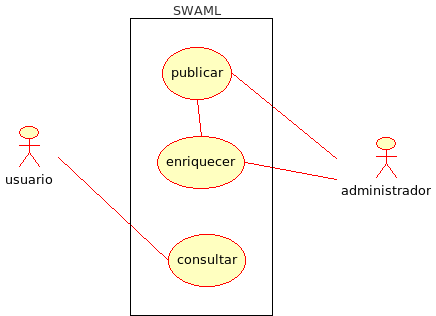
\includegraphics[width=12cm]{images/uml/casos-uso/general.png}
	\caption{Casos generales de uso}
	\label{uml:casos-uso}
\end{figure}

Como se ve en la figura~\ref{uml:casos-uso} se puede disntiguir claramente
tres grandes bloques de casos de uso:

\begin{itemize}
 \item Publicar los datos
 \item Enriquecerlos
 \item Consultarlos
\end{itemize}

\subsubsection{Casos de uso}

Refinando el diagrama anterior se identifican varios casos de uso que paso a
enumerar:

\begin{itemize}
 \item Parametrizar el sistema
 \item Iniciar la publicación
 \item Enriquecer los datos
 \item Consular los archivos generados
 \item Consultar la información extra generada
\end{itemize}

Para pasar a describirlos más detalladamente:

\begin{itemize}

  \item \textbf{Parametrizar el sistema:}
 	\begin{itemize}
 	  \item \textbf{Descripción:} Este caso de uso representa la labor 
		que el usuario administrador debe realizar para configurar 
		correctamente el sistema.
 	  \item \textbf{Flujo de eventos:} El caso de uso comienza cuando el
		usuario administrador comienza a editar una configuración, 
		bien manualmente o mediante el asistente que acompaña al 
		software.
	  \item \textbf{Precondiciones:} Es necesario disponer de un mailbox
		a exportar.
	  \item \textbf{Postcondiciones:} Ninguna detectada.
	\end{itemize}

  \item \textbf{Iniciar la publicación:}
 	\begin{itemize}
 	  \item \textbf{Descripción:} Representa la acción de publicación 
		propiamente dicha.
 	  \item \textbf{Flujo de eventos:} El proceso es un proceso por 
		lotes que a partir de una configuración genera una serie 
		de ficheros RDF. Internamente se divide en varios procesos:
		\begin{enumerate}
		 \item \emph{Parsear} el mailbox
		 \item Revisar la consistencia de todas las relaciones entre los distintos mensajes
		 \item Enriquecer la información
		 \item Exportar cada uno de estos mensajes en RDF
		 \item Exportar los suscriptores en RDF
		 \item Exportar los suscriptores en KML si fuese requerido
		 \item Exportar todos los indices
		\end{enumerate}
	  \item \textbf{Precondiciones:} Disponer de una configuración correcta.
	  \item \textbf{Postcondiciones:} El directorio destino de la exportación
		debe poder \emph{consumirse} mediante otro servicio, como un 
		servidor \texttt{HTTP} (Apache o similar).
	\end{itemize}

  \item \textbf{Enriquecer los datos:}
 	\begin{itemize}
 	  \item \textbf{Descripción:} Representa la interacción del 
		sistema con otras bases del conocimiento externas, 
		principalmente los FOAF de los suscriptores a la lista 
		de correo, para enriquecer la información en determinados 
		aspectos.
 	  \item \textbf{Flujo de eventos:} Se tratar de un proceso que se 
		repite iterativamente con cada uno de los suscriptores:
		\begin{enumerate}
		 \item Buscar su FOAF
		 \item Si lo tiene:
		 \begin{enumerate}
		  \item	Enlazar al suscriptor con su FOAF
		  \item Consultar sus coordenadas geográficas
		  \item Consultar su foto
		 \end{enumerate}
		 \item Si no lo tiene continuar con el siguiente suscriptor
		\end{enumerate}
	  \item \textbf{Precondiciones:} Disponer de la lista de suscriptores 
		cargada en memoria.
	  \item \textbf{Postcondiciones:} Ninguna detectada.
	\end{itemize}

  \item \textbf{Consular los archivos generados:}
 	\begin{itemize}
 	  \item \textbf{Descripción:} Representa la interacción del 
		usuario con los datos generados. Desde una simple consulta 
		manual a los ficheros RDF generados, hasta realizar consultas 
		de una forma más sofisticada.
 	  \item \textbf{Flujo de eventos:} Con la información obtenida se 
		repetirá siempre el mismo flujo:
		\begin{enumerate}
		 \item consultar
		 \item leer
		 \item comprender
		 \item y/o desechar
		\end{enumerate}
	  \item \textbf{Precondiciones:} Disponer de la lista exportada a RDF.
	  \item \textbf{Postcondiciones:} Ninguna concreta.
	\end{itemize}

  \item \textbf{Consultar la información extra generada:}
 	\begin{itemize}
 	  \item \textbf{Descripción:} Este caso de uso representa la consulta 
		por parte del usuario de la información extra generada, por el 
		ejemplo los suscriptores en formato KML.
 	  \item \textbf{Flujo de eventos:}
		\begin{enumerate}
		 \item consultar
		 \item explotar
		\end{enumerate}
	  \item \textbf{Precondiciones:} Disponer de la información geográfica 
		de los suscriptores.
	  \item \textbf{Postcondiciones:} Explotación de estos datos, por ejemplo
		visualizandolos\footnote{\url{http://maps.google.es/maps?q=http://swaml.berlios.de/demo/subscribers.kml}}
		con Google Maps\footnote{\url{http://maps.google.es/}}.
	\end{itemize}

\end{itemize}






\subsection{Especificaciones secundarias}

\subsubsection{Requisitos del sistema} 

El software no debera necesitar de unos requerimientos hardware elevados, 
siendo capaz de ejecutarse en un procesador de como mínimo 300Mhz, con 
un mínimo de 32Mb de memoria RAM. 

Los requisitos concretos (procesador de 32 o 64 bits, sistema operativo, 
etc) vendrán determinados por las inherentes restricciones del entorno de 
ejecución escogido para el proyecto.

\subsubsection{Requisitos de documentación} 

La documentación aportada deberá contener manuales para un completo uso 
del software entregado.

Al menos los siguientes tres documentos:

\begin{itemize}
  \item \textbf{Manual técnico} en el que se recoja toda la información que 
	fuera necesaria si un futuro se desea extender parte o la totalidad 
	del software por parte de personas totalmente ajenas al equipo de 
	desarrollo original.
  \item \textbf{Manual de despliegue} describiendo detalladamente todos los 
	requisitos previos y los pasos concretos que se deben seguir para la 
	correcta instalación del software.
  \item \textbf{Manual de usuario} que recoja ayuda detallada en un lenguaje
	no técnico para la correcta utilización del software.
\end{itemize}

Todos los documentos deberán, además de ser entregados impresos en papel a la
hora de entrega del resto de componentes del proyecto, estar disponibles en
formato imprimible (como por ejemplo PDF) en el sitio web público del proyecto.



\subsection{Plan del proyecto}

\subsubsection{Estimación de recursos}

\begin{itemize}

  \item \textbf{ Materiales:}
	\begin{table}[H]
	 \begin{center}
	  \begin{tabular}{|l|l|c|c|}
		\hline
		\textbf{ID Unidad} & \textbf{Descripción} & \textbf{Unidad de medición} & \textbf{Nº de unidades} \\
		\hline
		HW1 & Ordenador de tipo PC & unidad & 1 \\
		\hline
		SW1 & S.O. GNU/Linux & unidad & 1 \\
		\hline
		SW2 & Intérprete de Python & unidad & 1 \\
		\hline
		SW3 & Entorno de desarrollo Eclipse & unidad & 1 \\
		\hline
	  \end{tabular}
	  \caption{Recursos materiales}
	 \end{center}
	\end{table}

  \item \textbf{Personales:}
	\begin{table}[H]
	 \begin{center}
	  \begin{tabular}{|l|l|c|c|}
		\hline
		\textbf{ID Unidad} & \textbf{Descripción} & \textbf{Unidad de medición} & \textbf{Nº de unidades} \\
		\hline
		HU1 & Análisis y diseño & horas & 130 \\
		\hline
		HU2 & Desarrollo del software & horas & 380 \\
		\hline
		HU3 & Dirección técnica & horas & 42 \\
		\hline
	  \end{tabular}
	  \caption{Recursos personales}
	 \end{center}
	\end{table}

\end{itemize}


\subsubsection{Etapas del proyecto}

El desarrollo del proyecto ha quedado delimitado en varias etapas claramente
marcadas.

Las principales etapas, también recogidas en el gráfico de gantt de la 
figura~\ref{fig:gantt}, se enumeran en la siguiente tabla:


\begin{table}[H]
 \begin{center}
  \begin{tabular}{|l|l|c|c|}
	\hline
	\textbf{WBS} & \textbf{Tarea} & \textbf{Inicio} & \textbf{Fin} \\
	\hline
	\textbf{1}   & \textbf{Especificación de requisitos y estudio de viabilidad} & 26/09/2005 & 09/01/2006 \\
	\hline
	\textbf{2}   & \textbf{Análisis y Diseño} & 09/01/2006 & 15/02/2006 \\
	\hline
	\textbf{3}   & \textbf{Desarrollo Software} & 19/01/2006 & 21/11/2006 \\
	\textbf{3.1} & Desarrollo del core de SWAML & 19/01/2006 & 18/08/2006 \\	
	\textbf{3.2} & Desarrollo de Buxon & 18/08/2006 & 01/11/2006 \\
	\textbf{3.3} & Desarrollo de herramientas complementarias & 07/09/2006 & 21/11/2006 \\	
	\hline
	\textbf{4}   & \textbf{Elaboración de la documentación} & 01/06/2006 & 30/11/2006 \\	
	\hline
	\textbf{5}   & \textbf{Dirección} & 26/09/2005 & 01/12/2006 \\
	\hline
  \end{tabular}
  \caption{Planificación de las tareas}
 \end{center}
\end{table}

\begin{figure}[p]
 	\centering
	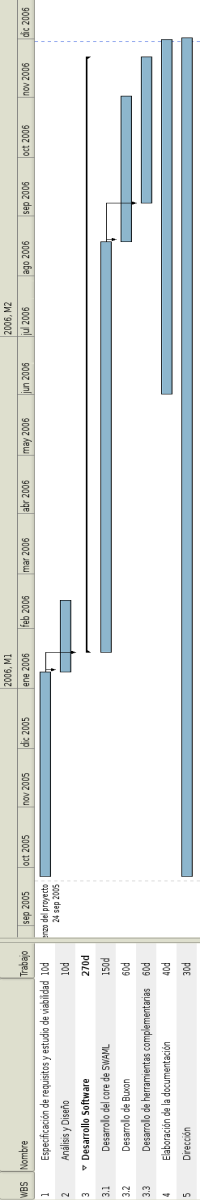
\includegraphics[width=4cm]{images/gantt.png}
	\caption{Planificación general del proyecto}
	\label{fig:gantt}
\end{figure}

\newpage

\subsubsection{Presupuesto}

\begin{itemize}

  \item \textbf{Tabla de precios:}
	\begin{table}[H]
	\begin{center}
	\begin{tabular}{|l|l|c|r|}
		\hline
		\textbf{ID Unidad} & \textbf{Descripción} & \textbf{Unidad de medición} & \textbf{Precio} \\
		\hline
		HW1 & Ordenador de tipo PC & \euro/ud & 1.190 \\
		\hline
		SW1 & S.O. GNU/Linux & \euro/ud & 0 \\
		\hline
		SW2 & Intérprete de Python & \euro/ud & 0 \\
		\hline
		SW3 & Entorno de desarrollo Eclipse & \euro/ud & 0 \\
		\hline
		HU1 & Análisis y diseño & \euro/h & 41,01 \\
		\hline
		HU2 & Desarrollo del software & \euro/h & 15,51 \\
		\hline
		HU3 & Dirección técnica & \euro/h & 59,85 \\
		\hline
	\end{tabular}
	\caption{Tabla de precios}
	\end{center}
	\end{table}

  \item \textbf{Presupuestos parciales:}
	\begin{table}[H]
	 \begin{center}
	  \begin{tabular}{|l|l|r|}
		\hline
		\textbf{ID Unidad} & \textbf{Descripción} & \textbf{Importe} \\
		\hline
		HW1 & Ordenador de tipo PC & 1.190,00 \euro \\
		\hline
		SW1 & S.O. GNU/Linux & 0,00 \euro \\
		\hline
		SW2 & Intérprete de Python & 0,00 \euro \\
		\hline
		SW3 & Entorno de desarrollo Eclipse & 0,00 \euro \\
		\hline
	  \end{tabular}
	  \caption{Presupuesto parcial de recursos materiales}
	 \end{center}
	\end{table}

	\begin{table}[H]
	 \begin{center}
	  \begin{tabular}{|l|l|r|}
		\hline
		\textbf{ID Unidad} & \textbf{Descripción} & \textbf{Importe} \\
		\hline
		HU1 & Análisis y diseño & 5.331,30 \euro \\
		\hline
		HU2 & Desarrollo del software & 5.893,80 \euro \\
		\hline
		HU3 & Dirección técnica & 2.513,70 \euro \\
		\hline
	  \end{tabular}
	  \caption{Presupuesto parcial de recursos personales}
	 \end{center}
	\end{table}	

  \item \textbf{Presupuesto final:}
	\begin{table}[H]
	 \begin{center}
	  \begin{tabular}{|l|r|}
		\hline
		\textbf{Descripción} & \textbf{Importe} \\ 
		\hline
		Recursos hardware & 1.190,00 \euro \\
		\hline
		Recursos software & 0,00 \euro \\
		\hline
		Recursos personales & 13.738,80 \euro \\
		\hline
		\textbf{SUBTOTAL} & \textbf{14.928,80 \euro} \\
		\hline
		Beneficio industrial (6\%) & 895,73 \euro \\
		\hline
		Costes generales (15\%) & 2.239,32 \euro \\
		\hline
		Suma de gastos y beneficios & 18.063,85 \euro \\
		\hline
		I.V.A. (16\%) & 2.890,22 \euro \\
		\hline
		\textbf{TOTAL} & \Large\textbf{20.954,06 \euro} \\
		\hline
	  \end{tabular}
	  \caption{Presupuesto final}
	 \end{center}
	\end{table}

\end{itemize}


